% Source : http://tex.stackexchange.com/questions/35526/tikz-tree-sibling-distance

\documentclass[landscape]{article}
	\usepackage[utf8]{inputenc}
	\usepackage[T1]{fontenc}
	\usepackage[margin=1in]{geometry}
	\usepackage{tikz-qtree}
	\usetikzlibrary{shadows,trees}
	
	\tikzset{
		font=\small,
		edge from parent fork down,
		level distance=1.75cm,
		every node/.style={
			top color=white,
			bottom color=blue!25,
			rectangle,
			rounded corners,
			minimum height=8mm,
			draw=blue!75,
			very thick,
			drop shadow,
			align=center
		},
		edge from parent/.style={
			draw=blue!50,
			thick
		}
	}


\begin{document}

\centering
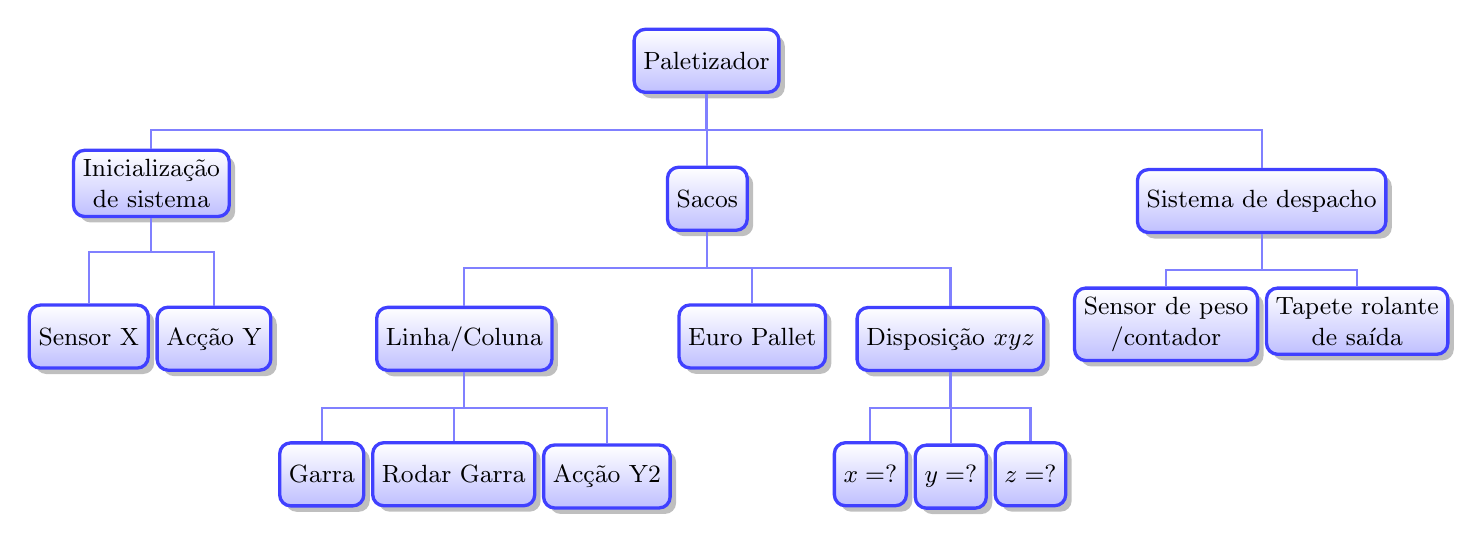
\begin{tikzpicture}
	\Tree [.Paletizador 
		[.{Inicialização\\de sistema}
			[.{Sensor X} ]
			[.{Acção Y} ]
		]
		[.Sacos
			[.{Linha/Coluna}
				[.{Garra} ]
				[.{Rodar Garra} ]
				[.{Acção Y2} ]
			]
			[.{Euro Pallet} ]
			[.{Disposição $xyz$}
				[.{$x=?$} ]
				[.{$y=?$} ]
				[.{$z=?$} ]
			]
		]
		[.{Sistema de despacho}
			[.{Sensor de peso\\/contador} ]
			[.{Tapete rolante\\de saída} ]
		]
]
\end{tikzpicture}

\end{document}


